%  %\PassOptionsToPackage{quiet}{xeCJK}
% %\PassOptionsToPackage{quiet}{fontspec}
% \documentclass{article}
% \usepackage[a4paper,left=3.18cm,right=3.18cm,top=2.54cm,bottom=2.54cm]{geometry}
% \usepackage[UTF8]{ctex}
% \usepackage{float}
% \usepackage{booktabs}
% \usepackage{verbatim}
% \usepackage{graphicx}
% %\usepackage{fontspec}
% %\setmainfont{Times New Roman}
% \setmainfont{XITS}
% \graphicspath{{fig/}}

% \title{绪论}
% \author{kraanium} %enter your name here
% \date{January 2023}
% \begin{document}
% \maketitle
\chapter*{绪论}
\section*{古诺尔斯语简介及其在语系中的定位}
古诺尔斯语(Old Norse)是北日耳曼语族的一个分支,发展自8世纪左右的原始诺尔斯语(Proto-Norse),在大约公元14世纪前,古诺尔斯语通行于斯堪地纳维亚居民以及维京人的海外殖民地。在维京人的口中,古诺尔斯语被称作dǫnsk tunga,意思是丹麦人的语言,这主要是因为当时民族认知的特性所致。由于其地理位置的影响,古诺尔斯语也被称作古冰岛语或古挪威语,甚至更宽泛的说法:古北欧语或者古斯堪地纳维亚语。只要不引起歧义,上述的说法都是可行的。不过,在更严格的术语定义下,古冰岛语、古挪威语都可算作古诺尔斯语的方言,只是二者的区别比较小。因此,古诺尔斯语是学术界更通行的用法。

古诺尔斯语隶属于日耳曼语族的北支,日耳曼语族又可分为三支:
\begin{enumerate}
    \item 北日耳曼语支。古代语言的代表即古诺尔斯语,在约公元14-15世纪后逐渐分化为现今的冰岛语、挪威语、瑞典语、丹麦语等。这些语言相似程度很高,除冰岛语尤其从古外,挪威语、瑞典语、丹麦语的书面语形式可以互通。这些现代语言在早期主要是古诺尔斯语的方言形式,关于这些方言的特征,参见下文。

    \item 西日耳曼语支。古代语言的代表是古英语、古高地德语、古撒克逊语、古法兰克语等。它们演化为今天的英语、德语和荷兰语等语言。西日耳曼语是日耳曼语族中最大的一支,在现存的约70种日耳曼语和方言中,只有6种属于北日耳曼语,其他均属于西日耳曼语。

    \item 东日耳曼语支。现已完全灭绝。古代语言的代表是哥特语,亦有零散的汪达尔语等的文本。东日耳曼语是日耳曼语族中最古老的一支,其文献记载是所有日耳曼语中最早的。哥特人曾大规模地向南移居过,因此在克里米亚地区保留了一支哥特人的部落,他们操克里米亚哥特语,但18世纪后亦灭绝。
\end{enumerate} 

在古代日耳曼语中,比较有代表性的是古英语(Old English,OE)、古高地德语(Old High German,OHG),古诺尔斯语和哥特语(Gothic,Go.),这些语言保留了十分充分的文本资料,在必要的情况下,本书将引用它们和古诺尔斯语进行比较。

这几种语言活跃的时间如下表所示:

\begin{table}[H]
\centering
\begin{tabular}{@{}ccc@{}}
\toprule
\textbf{语言} & \textbf{谱系} & \textbf{时间} \\ \midrule
哥特语         & 东日耳曼语       & 3-10世纪      \\
古英语         & 西日耳曼语       & 5-12世纪      \\
古高地德语       & 西日耳曼语       & 8-11世纪      \\
古诺尔斯语       & 北日耳曼语       & 8-15世纪      \\ \bottomrule
\end{tabular}
\end{table}

按照历史语言学的基本观点,所有日耳曼语都演变自一个共同的祖先——原始日耳曼语(Proto-Germanic,PGmc.)。原始语是一种拟构出来的,没有文字资料证实的假象语言,它对于揭示语言间的关联有着重要的作用。原始日耳曼语从一种更加古老、也更加重要的原始语中分化出来,后者称为原始印欧语(Proto-Indo-European,PIE)。原始印欧语和原始日耳曼语的规则都比较复杂,本书仅在必要的时候提供部分相关的知识,拟构出来的原始语用*标出,表示其未被证实存在。从原始日耳曼语中,东日耳曼语分化得最早,在音变等特征上相对比较保守;后分化的西日耳曼语和北日耳曼语则有一定的创新,例如规律的变元音(详见\ref{变元音})。西日耳曼语和北日耳曼语有一些共同的特征,因此一些学者认为它们来自一种原始西北日耳曼语,但尚无定论。

就古诺尔斯语本身而言,可以确定的是它从原始诺尔斯语演变而来。原始诺尔斯语大约流行于公元2-8世纪,虽然也称为“原始”,但与之前所述的原始印欧语和原始日耳曼语不同的是,原始诺尔斯语已经有了文字记载,但处于十分原始的阶段。原始诺尔斯语采用一种叫作卢恩文字的书写系统(区别于后期的拉丁字母),古代北欧人常将卢恩文字铭刻在石头、骨器上用以记录一些简单的信息,譬如人名、物品、祭祀时的祷告等。原始诺尔斯语的书写系统和书面记载都不发达,但它保留了许多词汇原本的特征。下图是卢恩字母表和卢恩石:

\begin{figure}[H]
    \centering
    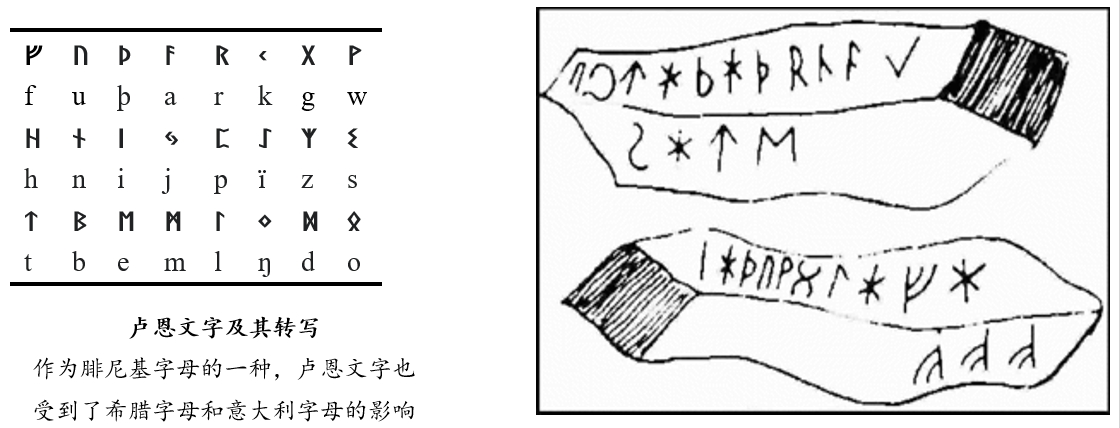
\includegraphics[width=\textwidth]{intro1.png}
\end{figure}

与之密切相关的一点是,卢恩字母在日耳曼文化中有着相当重要的地位,北欧神话中有关于卢恩字母神性的记载,因此在原始诺尔斯语消亡后,卢恩字母也伴随着拉丁字母(主要是基督教传入所致)一起使用了一段时间。

古诺尔斯语有三种方言,其中最重要的是其中的两种:古东诺尔斯语(Old East Norse)和古西诺尔斯语(Old West Norse)。前者演变出现今的丹麦语和瑞典语,后者演变出今天的挪威语、冰岛语、法罗语(丹麦属法罗群岛的官方语言,和冰岛语类似)。第三种方言称为古哥特兰语(Old Gutnish),是哥特兰岛(今属瑞典)民的语言。总体而言,古西诺尔斯语更有北日耳曼语的特点,即它相对于原始日耳曼语发生了更多的变化,而东诺尔斯语和哥特兰语则发展得相对保守。特别地,“哥特兰”一词的词根和“哥特”是完全一样的,哥特兰语也明显受到了哥特语的影响。另外,就文献记载而言,古西诺尔斯语的语料最为丰富,因此古西诺尔斯语是古诺尔斯语的主要方言。在不特别提及古诺尔斯语的方言时,古诺尔斯语一词本身主要指涉的也是古西诺尔斯语。在西诺尔斯语进一步演化的过程中,产生了两支主要的现代语言:冰岛语和挪威语。挪威语由于在斯堪的纳维亚半岛大陆上,与其他语言接触甚广,因此其语法与东诺尔斯语进化出的现代语言有类似之处。与之相反的是,冰岛语在相对闭塞的岛国上几乎不受影响地发展了800年,时至今日,现代冰岛语的语法和书面形式与古诺尔斯语仅有少量的区别。即便是没有受过任何语言学训练的人也能很快总结出冰岛语规则的形态学变化规律,例如阳性词尾-r在冰岛语中演化为了稍有区别的-ur,现代冰岛语的主要创新是语音上的。由于冰岛语良好的从古性,有时也用古冰岛语代替古诺尔斯语,这种说法的好处是可以显式地表达出这种语言的地理分布。

\section*{古诺尔斯语语法提要}

古诺尔斯语是一种屈折语,这意味它具有丰富的形态变化。可发生屈折变化的词类有名词、代词、指示词、形容词和动词。相比于几种古典的印欧语,例如拉丁文、希腊文和梵文,古诺尔斯语的屈折变化已经发生了大量简化。这与其说是古诺尔斯语的特点,倒不如说是日耳曼语的共性。日耳曼语在屈折上的最重要的创新是在动词系统上,具体来说,是用规则的构词法取代了原始印欧语相对复杂的变化。在音系上,北日耳曼语也有一些明显的创新,最主要的是变元音的使用。在古诺尔斯语中,变元音是一种比较规则的共时规律。

\subsection*{古诺尔斯语的音系}
本书使用的发音是约12世纪后的比较成熟的古诺尔斯语发音,它有9个单元音,每个都有长短之分。在标准的正字法中,在短音字母上加锐音符“ ˊ ”表示长元音。
这10个单元音用国际音标表示为:

\begin{table}[H]
\centering
\begin{tabular}{@{}ccccccccc@{}}
\toprule
    & \multicolumn{4}{c}{\textbf{前元音}}                          & \multicolumn{4}{c}{\textbf{后元音}}                          \\ \cmidrule(l){2-9} 
    & \multicolumn{2}{c}{非圆唇} & \multicolumn{2}{c}{圆唇} & \multicolumn{2}{c}{非圆唇} & \multicolumn{2}{c}{圆唇} \\ \cmidrule(l){2-9} 
高元音 & i          & iː         & y         & yː         &            &            & u         & uː         \\
中元音 & e          & eː         & ø         & øː         &            &            & o         & oː         \\
低元音 & ɛ          & ɛː         &           &            & a          & aː         & ɔ         & ɔː         \\ \bottomrule
\end{tabular}
\end{table}

古诺尔斯语另有三个双元音:/ɛi/, /ɔu/, /øy/

在元音系统中,最重要的一个特征是元音变异(Umlaut),以此法得到的元音称为变元音。元音变异指的是,后一音节的元音会影响前一音节中元音的性质,使前一个元音的性质趋向于后一个元音。元音变异是一种同化(Assimilation)现象,在北日耳曼语和西日耳曼语中比较常见,但完全不出现在东日耳曼语中。因此,这一定是一个相对比较晚的变化。

古诺尔斯语有两种元音变异:
\begin{enumerate}
    \item i-变异。后一音节中的i/j有把前一音节的元音抬高(Raising)、前置(Fronting)的趋向。例如把a抬高、前置到e,kraf- + -ja > krefja; gast- + -i > gesti.

    \item u-变异。后一音节中的u/w有把前一音节的元音圆唇化的趋向(Rounding)。例如把a圆唇化为ǫ(读作ɔ),barn- + -um > bǫrnum.
\end{enumerate}

除此之外,古诺尔斯语比较显著的共时规律是:
\begin{enumerate}
    \item 词中的半元音j/w根据后续元音的性质经常消失。

    \item 大量的辅音同化。

    \item 非重读元音经常省略。
\end{enumerate}

古诺尔斯语比较重要的历时规律是词尾音节的脱落,这时常导致造成变元音的i/u脱落。

\subsection*{动词}
古诺尔斯语的动词根据人称、数、时态、语态和语气发生变化,这种变化称为动词的变位(Conjugation)。古诺尔斯语有三个人称,分别是第一人称、第二人称和第三人称,和英语等一致;两个数,分别是单数和复数。PIE中原本还有双数,但在西北日耳曼语中完全消失了,仅在哥特语中还有保留;两个时态:现在时和过去时。其中PIE的现在时、将来时都合并到了古诺尔斯语的现在时,非现在时都合并到了过去式;两种语态:主动态和中动态;三种语气:直陈、虚拟和祈使。

古诺尔斯语基本的动词变位方法时根据人称、数、时态、语态和语气在动词词干后添加词尾,但一部分动词在过去时的变位中还需要改变词根中的元音。根据动词过去时的构成是否涉及元音的变换,可将动词分为两种:强动词和弱动词。

强动词的词根元音在过去时和过去分词中发生变换,类似于英语中sing-sang-sung这样的不规则动词。这种利用元音变化进行动词屈折的现象叫作元音交替(Ablaut)。元音交替是古老的语法现象,在PIE中非常常见,而且不同的交替模式(例如sing-sang-sung和run-ran-run是两种交替模式)比较复杂,在日耳曼语中,元音交替的模式基本固定为7大类。词根中的元音按这7种模式进行变换,构成了7类不同的变位法。

强动词继承了PIE中的元音交替,因而这些动词一般比较古老。新产生的动词不再适用元音交替这种规则,而是规则地加入一个塞音中缀构成过去时,这种动词称为弱动词。弱动词是日耳曼语的创新,有很强的构词力,因此弱动词是一个开放的类,新造的动词都按弱动词的方式变化;强动词是一个封闭的类,其数量基本已经固定,新动词不会再按照强动词变化,反而有一些强动词按类比的原则变成了弱动词。

古诺尔斯语中的弱动词塞音后缀是-ð-,英语中的对应是-ed(规则动词)。弱动词采用一套不同于强动词的词尾,根据其词尾的不同,还可以将弱动词分成3类,但其中区别相比强动词而言小得多。

古诺尔斯语还有一些不规则动词。一部分称为过去-现在混合动词,它们的现在时采用强动词的过去词尾,过去时按弱动词变位,这是PIE演化为PGmc.时造成的不对称现象。这类动词只有10个;还有一些如系动词这样的高度不规则动词。

\subsection*{名词、形容词和代词}
名词按照数和格发生变化。和动词类似,名词也只有单数和复数,双数已经完全消失;古诺尔斯语中有四个格:主格、属格、与格、宾格。格大略地可认为是名词在句子中充当的成分,相比与PIE的8个格,古诺尔斯语已经大量简化了名词格,因此一些格有比较复杂的用法。

名词还有两个不变的属性:一是名词的性,包括阴、阳、中三性;二是名词的变化方法,后者称为变格法。名词所属哪一种变格法和名词的性并不是一对一的关系,某些变格法涉及多个性的名词,同理,同属于一种性的名词又对应于不同的变格法。

变格法也分为两类,分别是强变格法和弱变格法,这个术语由动词系统类比而来。因此名词可分为强变化和弱变化名词。强变化名词曾经的词尾音节中有一个元音,例如a,o,i,按照元音的不同,又可以对强变化名词进一步分类;而弱变化名词曾经的词尾音节中不仅有一个元音,这个元音还总是接续一个鼻音n,如an,in. 类似地,也可以按元音的类别对弱变化名词进行划分。一共有5类强变化名词和3类弱变化名词。

古诺尔斯语中的名词可以添加一个-inn后缀使之称为特指名词,-inn相当于英文的the,但-inn要根据格、性、数发生变化,和下述的形容词有类似之处。一个名词是否是特指的在古诺尔斯语中有形态学上的作用,这会影响修饰它的形容词。

形容词和名词一样也要按数和格发生变化,但它还可以按性发生变化,即一个形容词可以变成阴、阳、中性。此外,形容词还可以根据它所修饰的名词是否为特指名词发生变化。此时可以把形容词的变格法分为强变格和弱变格两大类。如果修饰的名词是特指名词,要用形容词的弱变格形式,反之要用强变格形式。因此,一个形容词没有固定的属性,既没有固定的格、性、数,也没有固定的变格法。任何形容词都有两套变格法,要采取变格法中合适的形态使之与名词的格、性、数、特指性保持一致。

代词和形容词在语义和句法上的区别比较小,物主代词、指示代词、疑问代词等几乎都可以像形容词一样使用。因而代词与形容词有许多相似之处,很多形容词性的代词都按形容词的强变格法变化。但是,代词不区分特指性,因而没有强弱之分。

\section*{本书的结构}
TBD
